\chapter{Introduction}

Anyone reading this book should be familiar with the notion of the first, second and higher derivatives, \textit{e.g.},for $f(t) = t^3 + 5 t^2 + 2$, 
\begin{align}
  \frac{df}{dt}(t) &= 3 t^2 + 10 t \\
  \frac{d^2f}{dt^2}(t) &= 6t + 10 \\
  \label{eq:derivs}
\end{align}
\textit{etc.} Also we naturally think of integrals in an antiderivative sense, \textit{e.g.},
\begin{align}
  \int f(t) dt &= \frac{1}{4} t^4 + \frac{5}{3} t^3 + 5 t^2 + c 
  \label{eq:integrals}
\end{align}
and we adopt a notation of $f^{(1)}(t)$ as the first derivative, $f^{(2)}(t)$ as the second derivative and $f^{(n)}(t)$ as the $n$th derivative as well as $f^{(-1)}(t)$ as $f$ integrated one time, $f^{(-2)}$ as $f$ integrated two times, \textit{etc.}

A mathematically curious reader may already be wondering if there are any derivatives ``between'' the integer ones. For example, is the a one-half derivative:
\begin{equation}
  \frac{d^\frac{1}{d} f}{d t^\frac{1}{2}}(t) = f^{\left(\frac{1}{2}\right)} = ?.
  \label{eq:halfderiv}
\end{equation}
There is not an immediate obvious answer to this because of the fact that the integer order derivative (as is the integral) is defined as a limit
\begin{equation}
  \frac{df}{dt}(t) = \lim_{\Delta t \rightarrow 0} = \frac{f\left(t + \Delta t \right) - f\left(t\right)}{\Delta t}
  \label{eq:limdef}
\end{equation}
and that is a discrete operation. There is not a natural half way to do it.

Basically we want to gereralize the notion of the derivative. In a sense, if we define something to give the, say $\alpha$ derivative where $\alpha \in \mathbb R$, \textit{i.e.}, $\alpha$ is a real number, then all we really need is that when $\alpha$ is an integer we get the usual definition of that integer order derivative. In between there may be lots of different options (there are!), but it makes sense to set some other basic requirements we want a fractional-order derivative to satisfy.

\begin{example}
  Consider $f(t) = t^2$ with the first and second derivatives $f^{(1)}(t) = 2 t$ and $f^{(2)}(t) = 2$. We should expect that the $1/2$ derivative is, in some qualitative sense, ``between'' $f(t)$ and $f^{(1)}(t)$, and that the $3/2$ derivative is ``between'' the first and second derivatives. 

  % Title: gl2ps_renderer figure
% Creator: GL2PS 1.4.2, (C) 1999-2020 C. Geuzaine
% For: Octave
% CreationDate: Tue Jan 12 17:18:13 2021
\setlength{\unitlength}{1pt}
\begin{picture}(0,0)
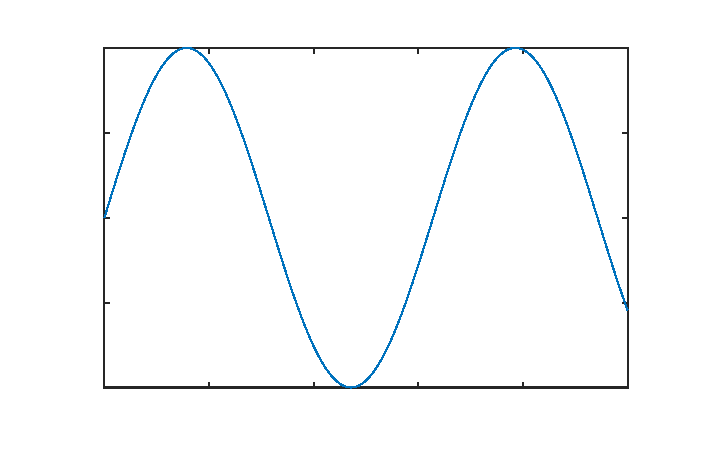
\includegraphics[scale=1]{fig-inc}
\end{picture}%
\begin{picture}(324,200)(0,0)
\fontsize{5}{0}\selectfont\put(42.12,17.7868){\makebox(0,0)[t]{\textcolor[rgb]{0.15,0.15,0.15}{{0}}}}
\fontsize{5}{0}\selectfont\put(92.34,17.7868){\makebox(0,0)[t]{\textcolor[rgb]{0.15,0.15,0.15}{{2}}}}
\fontsize{5}{0}\selectfont\put(142.56,17.7868){\makebox(0,0)[t]{\textcolor[rgb]{0.15,0.15,0.15}{{4}}}}
\fontsize{5}{0}\selectfont\put(192.78,17.7868){\makebox(0,0)[t]{\textcolor[rgb]{0.15,0.15,0.15}{{6}}}}
\fontsize{5}{0}\selectfont\put(243,17.7868){\makebox(0,0)[t]{\textcolor[rgb]{0.15,0.15,0.15}{{8}}}}
\fontsize{5}{0}\selectfont\put(293.22,17.7868){\makebox(0,0)[t]{\textcolor[rgb]{0.15,0.15,0.15}{{10}}}}
\fontsize{5}{0}\selectfont\put(39.3101,22){\makebox(0,0)[r]{\textcolor[rgb]{0.15,0.15,0.15}{{-1}}}}
\fontsize{5}{0}\selectfont\put(39.3101,62.75){\makebox(0,0)[r]{\textcolor[rgb]{0.15,0.15,0.15}{{-0.5}}}}
\fontsize{5}{0}\selectfont\put(39.3101,103.5){\makebox(0,0)[r]{\textcolor[rgb]{0.15,0.15,0.15}{{0}}}}
\fontsize{5}{0}\selectfont\put(39.3101,144.25){\makebox(0,0)[r]{\textcolor[rgb]{0.15,0.15,0.15}{{0.5}}}}
\fontsize{5}{0}\selectfont\put(39.3101,185){\makebox(0,0)[r]{\textcolor[rgb]{0.15,0.15,0.15}{{1}}}}
\end{picture}

\end{example}

% Title: gl2ps_renderer figure
% Creator: GL2PS 1.4.2, (C) 1999-2020 C. Geuzaine
% For: Octave
% CreationDate: Tue Jan 12 17:18:13 2021
\setlength{\unitlength}{1pt}
\begin{picture}(0,0)
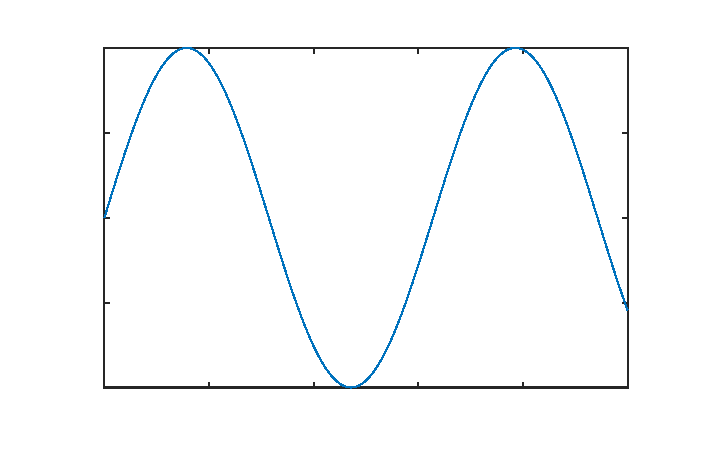
\includegraphics[scale=1]{fig-inc}
\end{picture}%
\begin{picture}(324,200)(0,0)
\fontsize{5}{0}\selectfont\put(42.12,17.7868){\makebox(0,0)[t]{\textcolor[rgb]{0.15,0.15,0.15}{{0}}}}
\fontsize{5}{0}\selectfont\put(92.34,17.7868){\makebox(0,0)[t]{\textcolor[rgb]{0.15,0.15,0.15}{{2}}}}
\fontsize{5}{0}\selectfont\put(142.56,17.7868){\makebox(0,0)[t]{\textcolor[rgb]{0.15,0.15,0.15}{{4}}}}
\fontsize{5}{0}\selectfont\put(192.78,17.7868){\makebox(0,0)[t]{\textcolor[rgb]{0.15,0.15,0.15}{{6}}}}
\fontsize{5}{0}\selectfont\put(243,17.7868){\makebox(0,0)[t]{\textcolor[rgb]{0.15,0.15,0.15}{{8}}}}
\fontsize{5}{0}\selectfont\put(293.22,17.7868){\makebox(0,0)[t]{\textcolor[rgb]{0.15,0.15,0.15}{{10}}}}
\fontsize{5}{0}\selectfont\put(39.3101,22){\makebox(0,0)[r]{\textcolor[rgb]{0.15,0.15,0.15}{{-1}}}}
\fontsize{5}{0}\selectfont\put(39.3101,62.75){\makebox(0,0)[r]{\textcolor[rgb]{0.15,0.15,0.15}{{-0.5}}}}
\fontsize{5}{0}\selectfont\put(39.3101,103.5){\makebox(0,0)[r]{\textcolor[rgb]{0.15,0.15,0.15}{{0}}}}
\fontsize{5}{0}\selectfont\put(39.3101,144.25){\makebox(0,0)[r]{\textcolor[rgb]{0.15,0.15,0.15}{{0.5}}}}
\fontsize{5}{0}\selectfont\put(39.3101,185){\makebox(0,0)[r]{\textcolor[rgb]{0.15,0.15,0.15}{{1}}}}
\end{picture}


